% ViT 1x make
% Author: Marcel Simader (marcel.simader@jku.at)
% Date: 04.11.2023
% License: See 'LICENSE'.

%            JJJJ   K                         K   UUUU         UUUU
%            JJJJ   KKKK                   KKKK   UUUU         UUUU
%            JJJJ   KKKKKK               KKKKKK   UUUU         UUUU
%            JJJJ      KKKKKK         KKKKKK      UUUU         UUUU
%            JJJJ         KKKKKK   KKKKKK         UUUU         UUUU
%            JJJJ            KKKKKKKKK            UUUU         UUUU
%    JJ     JJJJJ               KKK               UUUUU       UUUUU
%  JJJJJJJJJJJJJ    KKKKKKKKKKKKKKKKKKKKKKKKKKK    UUUUUUUUUUUUUUU
%    JJJJJJJJJ      KKKKKKKKKKKKKKKKKKKKKKKKKKK      UUUUUUUUUUU
%
% Template created by Susanne Hametner and Doris Pargfrieder
% Template altered by Pieter-Jan Hoedt (2020)
% Template rewritten by Michael Roland (2021)
% Template adapted by Marcel Simader (2023)

% ViT included in content.tex
% Author: Marcel Simader (marcel0simader@gmail.com)
% Date: 04.11.2023
% License: See 'LICENSE'.

% ~~~~~~~~~~~~~~~~~~~~~~~~~~~~~~~~~~~~~~~~~~~~~~~~~~~~~~~~
% ~~~~~~~~~~~~~~~~~~~~ Document Class ~~~~~~~~~~~~~~~~~~~~
% ~~~~~~~~~~~~~~~~~~~~~~~~~~~~~~~~~~~~~~~~~~~~~~~~~~~~~~~~

\documentclass[utf8, aspectratio=169, english]{beamer}
% Define the aspect ratio of the slide layout:
%  * aspectratio=169  ... 16:9 aspect ratio
%  * aspectratio=43   ... 4:3 aspect ratio
%  * aspectratio=1610 ... 16:10 aspect ratio
% Define document languages:
%  * ngerman ... German
%  * english ... English
%  * ...
% Switch to handout mode:
%  * handout ... A compact mode that allows you to remove animation and skips slides for
%                efficient printing.
% Other options:
%  * utf8 ... Treat input files as UTF-8 encoded. Make sure to always provide that option
%             when you use pdfLaTeX so that pdfLaTeX knows how to read and interpret
%             characters this source file.

\setbeamercovered{transparent}

% ~~~~~~~~~~~~~~~~~~~~~~~~~~~~~~~~~~~~~~~~~~~~~~~
% ~~~~~~~~~~~~~~~~~~~~ Theme ~~~~~~~~~~~~~~~~~~~~
% ~~~~~~~~~~~~~~~~~~~~~~~~~~~~~~~~~~~~~~~~~~~~~~~

%\usepackage[TNF,nosectionpage]{style/jku}
\usepackage[%
    darkmode, fancyfonts, mathastext,%
    framenumber, totalframenumber,%
    TNF, logopath={./style/logos},fontpath={./style/fonts}]{style/beamerthemejku}
% Color scheme selection options:
%  * JKU  ... Use JKU (gray) color scheme (this is the default if no scheme is selected).
%  * BUS  ... Use Business School color scheme.
%  * LIT  ... Use Linz Institute of Technology color scheme.
%  * MED  ... Use MED faculty color scheme.
%  * RE   ... Use RE faculty color scheme.
%  * SOE  ... Use School of Education color scheme.
%  * SOWI ... Use SOWI faculty color scheme.
%  * TNF  ... Use TNF faculty color scheme.
% Color mode selection options:
%  * darkmode ... Use dark color mode (where title and logo frames have a dark background).
% Frame numbering options:
%  * framenumber         ... Insert frame number into the frame footer.
%  * totalframenumber    ... Insert frame number and total frame number into the frame footer
%                            (only frames in the main part are counted).
%  * appendixframenumber ... Similar to `totalframenumber', but count the overall total frame
%                            number of main part and appendix.
% Note that combining `totalframenumber' and `appendixframenumber' options will show the total
% number of frames for the main part on frames in the main part and the overal total number of
% frames for frames in the appendix.
% Sectioning options:
%  * nosectionpage       ... Supress section frames (see \section{<title>} command).
%  * nosubsectionpage    ... Supress subsection frames (see \subsection{<title>} command).
%  * nosubsubsectionpage ... Supress subsubsection frames (see \subsubsection{<title>} command).
%  * partpage            ... Insert part frames (see \part{<title>} command).
% Space-efficient monospace font options (requires XeTeX):
%  * compactmono   ... Use condensed fixed-width font everywhere.
%  * nocompactverb ... Do not use condensed fixed-width font for verbatim and listings.
% Style-breaking options:
%  * nojkufooter    ... Do not insert JKU/partner logos into the frame footer.
%  * nofooter       ... Do not display a frame footer.
%  * noimprint      ... Do not insert imprint on title pages.
%  * nojkulogo      ... Do not insert JKU & K logos on title pages and in frame footers.
%  * frametitlecaps ... Set frame titles in capital letters (like in eariler theme versions).
%  * nofancyfonts   ... Do not use custom TTF fonts with XeTeX / supress pdfLaTeX warning.
%  * mac            ... Use adapted color palette for screen display on Mac.
%  * legacyitemizestyle ... Use old bullet style in itemization.
% Experimental options:
%  * mathastext ... Use standard document fonts (and default to sans-serif font) in math mode
% Advanced options:
%  * nooptpackages     ... Do not load additional convenience packages (which are only there
%                          to provide interoperability to the behavior of previous versions of
%                          this theme but are not actually required for the current version).
%  * logopath={<path>} ... Set the path where the theme can find its own logo resources. This
%                          should typically be a relative path and the default is `./logos'.
%  * fontpath={<path>} ... Set the path where the theme can find its own font resources. This
%                          should typically be a relative path and the default is `./fonts'.

% ~~~~~~~~~~~~~~~~~~~~~~~~~~~~~~~~~~~~~~~~~~~~~~~~~~~~~~~~~~~
% ~~~~~~~~~~~~~~~~~~~~ Included Packages ~~~~~~~~~~~~~~~~~~~~
% ~~~~~~~~~~~~~~~~~~~~~~~~~~~~~~~~~~~~~~~~~~~~~~~~~~~~~~~~~~~

% Default stuff...
\usepackage{xspace}
\usepackage{multicol}
\usepackage{hyperref}
\usepackage{csquotes}
% \usepackage{pifont}
% \usepackage{bold-extra}
\usepackage{xcolor}
% \usepackage{caption}
\usepackage{acronym}
% \usepackage[acronym]{glossaries}
\usepackage{environ}

% Maths stuff...
\usepackage{amssymb}
\usepackage{mathtools}
\usepackage{amsthm}

% Table stuff...
\usepackage{booktabs}
% \usepackage{tabularx}
% \usepackage{threeparttable}

% Tikz stuff...
% \usepackage{tikz}
% \usetikzlibrary{shapes.geometric}
% \usetikzlibrary{positioning}

% Float figure stuff...
\usepackage{listings}
% \usepackage{wrapfig}
% \setlength{\columnsep}{20pt}

% BibLaTeX stuff...
\usepackage[%
    backend=biber,sortcites=true,%
    style=style/ACM-Reference-Format]{biblatex}
\preto{\bibsetup}{\providecommand*{\insertbiblabel}{}}
\DeclareFieldFormat*{title}{#1}
\DeclareFieldFormat*{booktitle}{#1}
\DeclareFieldFormat*{journaltitle}{#1}
\setcounter{biburlnumpenalty}{100}
\setcounter{biburllcpenalty}{100}
\setcounter{biburlucpenalty}{100}
\addbibresource{literature.bib}

% ~~~~~~~~~~~~~~~~~~~~~~~~~~~~~~~~~~~~~~~~~~~~~~~~
% ~~~~~~~~~~~~~~~~~~~~ Macros ~~~~~~~~~~~~~~~~~~~~
% ~~~~~~~~~~~~~~~~~~~~~~~~~~~~~~~~~~~~~~~~~~~~~~~~

\def\P(#1){\ensuremath{P\mkern-0.5mu\left( #1 \right)}}

\NewEnviron{m-question}{%
    \begingroup
    \setbeamercolor{block title}{fg=white,bg=jkuPurple}
    \begin{block}{Research Question}
        \begin{displayquote}
            \large\vspace*{0.25\baselineskip}%
            \openautoquote{\BODY}\closeautoquote%
            \vspace*{0.2\baselineskip}
        \end{displayquote}
    \end{block}
    \endgroup}

\NewEnviron{m-problem}{%
    \begingroup
    \setbeamercolor{block title}{fg=white,bg=jkuRed}
    \begin{block}{Problem}
        \large\vspace*{0.25\baselineskip}{\BODY}\vspace*{0.2\baselineskip}
    \end{block}
    \endgroup}


% ~~~~~~~~~~~~~~~~~~~~~~~~~~~~~~~~~~~~~~~~~~~~~~~~~~~~~~~~
% ~~~~~~~~~~~~~~~~~~~~ Begin Document ~~~~~~~~~~~~~~~~~~~~
% ~~~~~~~~~~~~~~~~~~~~~~~~~~~~~~~~~~~~~~~~~~~~~~~~~~~~~~~~

\begin{document}

% Settings {{-{
% ~~~~~~~~~~~~~~~~~~~~~~~~~~~~~~~~~~~~~~~~~~~~~~~~~~
% ~~~~~~~~~~~~~~~~~~~~ Settings ~~~~~~~~~~~~~~~~~~~~
% ~~~~~~~~~~~~~~~~~~~~~~~~~~~~~~~~~~~~~~~~~~~~~~~~~~

% Acronyms {{-{
% ~~~~~~~~~~~~~~~~~~~~ Acronyms ~~~~~~~~~~~~~~~~~~~~
\newacro{AI}[AI]{Artificial Intelligence}
\newacro{ML}[ML]{Machine Learning}
\newacro{NLP}[NLP]{Natural Language Processing}
\newacro{LM}[LM]{Language Model}
\newacro{LLM}[LLM]{Large Language Model}
\newacro{NN}[NN]{Neural Network}
\newacro{DNN}[DNN]{Deep Neural Network}
\newacro{RNN}[RNN]{Recurrent Neural Network}
\newacro{LSTM}[LSTM]{Long Short-Term Memory}
\newacroplural{LSTM}[LSTMs]{Long Short-Term Memory Models}
\newacro{BPE}[BPE]{Byte Pair Encoding}
\newacro{OOV}[OOV]{Out of Vocabulary}
\newacro{LBL}[LBL]{Logbilinear}
\newacro{GPT}[GPT]{Generative Pre-Trained Transformer}
% }-}}

% Title Page {{-{
% ~~~~~~~~~~~~~~~~~~~~ Title Page ~~~~~~~~~~~~~~~~~~~~
% ~~~~~~~~~~~~~~~~~~~~ Series Title ~~~~~~~~~~~~~~~~~~~~

% Command \series{series title}: sets the series title
\series{PAT'24}

% ~~~~~~~~~~~~~~~~~~~~ Title ~~~~~~~~~~~~~~~~~~~~

% Command \title[short title]{title}: sets the presentation title
% Command \titlesmall{text}: switches to small font size inside title
\title[Identifier Quality Metrics]{Measuring Identifier Quality\\ with \acl{ML}}
\acused{ML}

% ~~~~~~~~~~~~~~~~~~~~ Subtitle ~~~~~~~~~~~~~~~~~~~~

% Command \subtitle[short subtitle]{subtitle}: sets the presentation subtitle
\subtitle[A Survey]{A Survey of Existing Approaches}

% ~~~~~~~~~~~~~~~~~~~~ Author ~~~~~~~~~~~~~~~~~~~~

% Command \author[short authors]{authors}: sets the presentation authors (multiple authors
% may be separated with \and)
\author[Simader \and Frischherz]{Marcel Simader \and Melissa Frischherz}

% ~~~~~~~~~~~~~~~~~~~~ Institute ~~~~~~~~~~~~~~~~~~~~

% Command \institute{name}: sets the institute / author affiliation (style-breaking)
% \institute{Institute for Symbolic Artificial Intelligence}
% Command \institutecode{CODE}: sets the institute abbreviation/initials (used to load the
% institute logo file, if present)
% \institutecode{SAI}

% ~~~~~~~~~~~~~~~~~~~~ Date ~~~~~~~~~~~~~~~~~~~~

% Command \date[short date]{date}: sets the presentation date (short date is used in the
% footer by default)
\date[2024-06-12]{}  % use this to set the date on the title page and in the footer
% \date[\today]{} % use this to set the date except for the title page

% ~~~~~~~~~~~~~~~~~~~~ Partner Logo ~~~~~~~~~~~~~~~~~~~~

% Command \partnerlogo[white=filename]{filename}: use filename as partner logo (leave
% filename blank to disable the partner logo), the optional argument ``white='' defines a
% separate file for use on dark background
% \partnerlogo{our_partner_logo}
% }-}}

% ~~~~~~~~~~~~~~~~~~~~ Footer ~~~~~~~~~~~~~~~~~~~~

% Command \footer{text}: sets the footer field
\footer{\expandafter\notblank\expandafter{\insertsectionhead}{%
    \insertsectionhead\expandafter\notblank\expandafter{\insertsubsectionhead}{%
        ~--~\insertsubsectionhead%
    }{}}{}}
% \footer{\insertshorttitle}  % a good alternative

% Command \footerdate{text}: sets the footer date field
\footerdate{\insertshortdate} % the default

% Command \footerpartnerlogo{filename}: use a different partner logo in the footer (e.g.
% a logo with a different form factor or no filename to disable the partner logo in the
% footer)
% \footerpartnerlogo{our_partner_logo}

% ~~~~~~~~~~~~~~~~~~~~ Agenda ~~~~~~~~~~~~~~~~~~~~

% Command \agenda[caption]{text}: sets the agenda (and optional caption) to display on the
% next title or section page
% \agenda{LIT AI Lab Gathering}

% }-}}

% Begin Frames {{-{
% ~~~~~~~~~~~~~~~~~~~~~~~~~~~~~~~~~~~~~~~~~~~~~~~~~~~~~~
% ~~~~~~~~~~~~~~~~~~~~~~~~~~~~~~~~~~~~~~~~~~~~~~~~~~~~~~
% ~~~~~~~~~~~~~~~~~~~~~~~~~~~~~~~~~~~~~~~~~~~~~~~~~~~~~~
% ~~~~~~~~~~~~~~~~~~~~ Begin Frames ~~~~~~~~~~~~~~~~~~~~
% ~~~~~~~~~~~~~~~~~~~~~~~~~~~~~~~~~~~~~~~~~~~~~~~~~~~~~~
% ~~~~~~~~~~~~~~~~~~~~~~~~~~~~~~~~~~~~~~~~~~~~~~~~~~~~~~
% ~~~~~~~~~~~~~~~~~~~~~~~~~~~~~~~~~~~~~~~~~~~~~~~~~~~~~~

\maketitle
% options:
%  * light ... use light color theme
%  * dark  ... use dark color theme
%  * gray  ... use JKU gray color theme
%  * black ... use black background
% In addition, options may contain a faculty name (see theme options) to
% use the faculty's color theme, e.g. `\maketitle[LIT,dark]'.

% Introduction {{-{
% ~~~~~~~~~~~~~~~~~~~~~~~~~~~~~~~~~~~~~~~~~~~~~~~~~~~~~~
% ~~~~~~~~~~~~~~~~~~~~ Introduction ~~~~~~~~~~~~~~~~~~~~
% ~~~~~~~~~~~~~~~~~~~~~~~~~~~~~~~~~~~~~~~~~~~~~~~~~~~~~~

\section*{Introduction}
\label{sec:Introduction}

% Overview {{-{
% ~~~~~~~~~~~~~~~~~~~~ Overview ~~~~~~~~~~~~~~~~~~~~
\subsection{Overview}
\label{ssec:Overview}

\begin{frame}{Overview}
    \vfill
    \begin{m-question}
        What \acl{ML} techniques exist to (automatically) measure the quality of
        identifiers?
    \end{m-question}
    \vfill
\end{frame}

\imageframe{A source code identifier is:}%
    {\begin{itemize}
        \setlength{\itemsep}{1.4ex}
        \item a textual name for something.
        \item a dense unit of semantic information.
        \item difficult to come up with!
    \end{itemize}}%
    {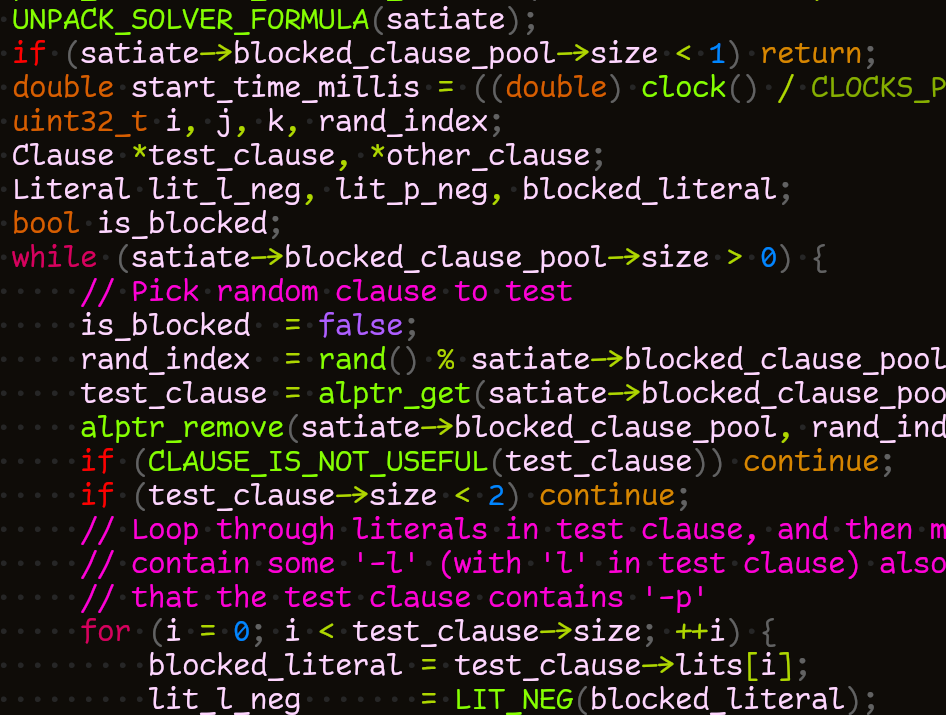
\includegraphics[height=\paperheight]{media/source-code.png}}

\begin{frame}{Overview}
    \begin{m-question}
        Why is identifier quality important in the software engineering context?
    \end{m-question}

    \pause % ~~~~~~~~~~~~~~~~~~~~~~~~~~~~~~~~~~~ PAUSE ~~~~~~~~~~~~~~~~~~~~~~~~~~~~~~~~~~~

    \begin{itemize}
        \item

        Identifiers make up ca.\@ 70\% of all source code~\cite{Gao2019IdentGen}

        \item

        Poor choices for identifiers lead to:

        \begin{tightlist}
            \begin{itemize}
            \item less readable code
            \item less maintainable code
            \item overall worse quality code~\cite{Butler2010Empirical}
            \end{itemize}
        \end{tightlist}

        \item

        Naming things is hard, because the name must \emph{describe the meaning}

    \end{itemize}
\end{frame}

% }-}}

% Methodology {{-{
% ~~~~~~~~~~~~~~~~~~~~ Methodology ~~~~~~~~~~~~~~~~~~~~
\subsection{Methodology}
\label{ssec:Methodology}

\begin{frame}{Methodology}
    \begin{multicols}{2}
        \begin{itemize}
            \setlength{\itemsep}{1.1ex}

            \item

            We analyzed 34 papers in total, selected 7 for detailed analysis

            \item

            Exploration on Elicit~\cite{elicit}, Google Scholar~\cite{googlescholar}, and
            IEEEXplore~\cite{ieeexplore}

            \item

            Search queries can be found in the paper

            \item

            We suspect the large increase around 2019 is due to Google's famous
            \citetitle{Vaswani2017Transformer} paper

        \end{itemize}

        \newcolumn

        \begin{figure}[h!]
            \begin{tikzpicture}[scale=0.8]
                \begin{axis}[%
                    ybar, bar width=6.5pt, ylabel={\# Publications}, xlabel={Year},
                    enlargelimits=0.03,
                    symbolic x coords={1999, 2000, 2001, 2002, 2003, 2004, 2005, 2006,%
                                       2007, 2008, 2009, 2010, 2011, 2012, 2013, 2014,%
                                       2015, 2016, 2017, 2018, 2019, 2020, 2021, 2022,%
                                       2023, 2024}]
                     \addplot+[y filter/.expression={y==0 ? nan : y}, line width=0.2pt]%
                        table [col sep=comma, header=true]%
                        {./data/ext-pubdates.csv};
                \end{axis}
            \end{tikzpicture}
            \caption{Histogram of Survey Paper Publications}
            \label{fig:Histogram-of-Survey-Paper-Publications}
        \end{figure}

    \end{multicols}
\end{frame}
% }-}}

% }-}}

% Survey {{-{
% ~~~~~~~~~~~~~~~~~~~~~~~~~~~~~~~~~~~~~~~~~~~~~~~~
% ~~~~~~~~~~~~~~~~~~~~ Survey ~~~~~~~~~~~~~~~~~~~~
% ~~~~~~~~~~~~~~~~~~~~~~~~~~~~~~~~~~~~~~~~~~~~~~~~

\section*{Survey}
\label{sec:Survey}

% NLP {{-{
% ~~~~~~~~~~~~~~~~~~~~ NLP ~~~~~~~~~~~~~~~~~~~~
\subsection{\acl{NLP}}
\label{ssec:Survey-NLP}

\begin{frame}{\acl{NLP}}
    \begin{m-problem}
        Extracting the information contained within an identifier is very difficult!
    \end{m-problem}

    \vspace*{\baselineskip}

    \begin{itemize}
        \setlength{\itemsep}{1ex}
        \item

        \acfa{NLP} is the analysis of language as humans speak it

        \item

        Research on \acs{NLP} active since the 1990s, proposed as early as the
        1950s~\cite{Brown1990StatMT}

    \end{itemize}

\end{frame}

\begin{frame}{\acl{NLP}}
    \begin{definition}
        The general goal of \acs{NLP} is to find the probability of some word $s_i$
        occurring in a sentence $s_1\:s_2 \ldots s_i\;$:\vspace{-0.6ex}
        \begin{equation*}
            \P(s_1\:s_2 \ldots s_i)
                = \P(s_1) \P(s_2 \mid s_1)
                \cdots \P(s_i \mid
                    \smash[b]{\underbrace{s_1 \ldots s_{i-1}}_{\text{\enquote{Context}}}})
                \text{~\cite{Brown1990StatMT}.}
        \end{equation*}
        \vspace{-0.7ex}
    \end{definition}

    \pause % ~~~~~~~~~~~~~~~~~~~~~~~~~~~~~~~~~~~ PAUSE ~~~~~~~~~~~~~~~~~~~~~~~~~~~~~~~~~~~

    \begin{itemize}
        \setlength{\itemsep}{1ex}
        \item

        We cannot compute all of these probabilities

        \item

        Context information must be condensed, somehow

        \item

        \citeauthor*{Zhang2023RenamingPrediction} use a random forest classifier with
        heuristic metrics to approximate these
        probabilities~\cite{Zhang2023RenamingPrediction}

    \end{itemize}
\end{frame}

\begin{frame}{\acl{NLP} with $n$-Grams}
    \begin{itemize}
        \item

        The $n$-gram model \enquote{chops off} the tail of the probability distribution

    \end{itemize}

    \begin{example}
        For $n = 2$ (\enquote{bigram}), the probability is now $\P(s_{i-1}\:s_i) =
        \P(s_{i-1}) \P(s_i \mid s_{i-1})$.
    \end{example}

    \pause % ~~~~~~~~~~~~~~~~~~~~~~~~~~~~~~~~~~~ PAUSE ~~~~~~~~~~~~~~~~~~~~~~~~~~~~~~~~~~~

    \begin{m-problem}
        This works well for machine translation, but we cannot handle \acfa{OOV}
        words\ldots~\cite{Shi2022Splitting,Allamanis2015Suggesting}
    \end{m-problem}

    \begin{itemize}
        \item

        Idea: Split identifiers into tokens (e.g.\@
        \texttt{get}~\slash~\texttt{Root}~\slash~\texttt{State}) \\
        $\Longrightarrow$ fewer (new) words in training
        set~\cite{Shi2022Splitting,Karampatsis2020BPE,Allamanis2015Suggesting}

    \end{itemize}
\end{frame}

% }-}}

% Neural Networks {{-{
% ~~~~~~~~~~~~~~~~~~~~ Neural Networks ~~~~~~~~~~~~~~~~~~~~
\subsection{\aclp{NN}}
\label{ssec:Survey-NN}

\begin{frame}{\aclp{NN} and \aclp{DNN}}
    \begin{description}[\acfp{DNN}:]
        \setlength{\itemsep}{1.05ex}

        \item[\acfp{NN}:]

        Based on the neuron, one input and one output layer

        \item[\acfp{DNN}:]

        Have at least one \enquote{hidden layer} of neurons \\
        \emph{$\Longrightarrow$ model of the human brain}

    \end{description}

    \vspace*{\baselineskip}

    \begin{itemize}
        \setlength{\itemsep}{1.05ex}
        \item

        \acsp{NN} generally offer better accuracy for \acs{NLP} applications

        \item

        We can now approximate the probability $\P(s_1\:s_2 \ldots s_i)$ directly!
    \end{itemize}
\end{frame}

\begin{frame}{\aclp{NN} and \aclp{DNN}}
    \begin{itemize}
        \setlength{\itemsep}{1ex}
        \item

        \citeauthor*{Allamanis2015Suggesting} propose the \acfa{LBL} \acfa{LM} as solution
        to the $n$-grams limitations

        \item

        They show that their solution \enquote{substantially outperforms} the $n$-gram for
        method and type names~\cite{Allamanis2015Suggesting}

    \end{itemize}

    \pause % ~~~~~~~~~~~~~~~~~~~~~~~~~~~~~~~~~~~ PAUSE ~~~~~~~~~~~~~~~~~~~~~~~~~~~~~~~~~~~

    \vspace*{\baselineskip}

    \begin{m-problem}
        \acsp{NN} and \acsp{DNN} are not well-suited for \emph{sequential inputs}, since
        the input layer must scale linearly with the sequence length.
    \end{m-problem}
\end{frame}

\begin{frame}{\aclp{RNN}}
    \begin{description}[\acfp{RNN}:]
        \setlength{\itemsep}{1.05ex}

        \item[\acfp{RNN}:]

        Can handle a sequential input by tracking and evaluating its own state \\
        \emph{$\Longrightarrow$ model of human memory}

        \item[\acfa{LSTM}:]

        Improved kind of \acs{RNN} presented by~\citeauthor{Hochreiter97LSTM}
        in~\citeyear{Hochreiter97LSTM}~\cite{Hochreiter97LSTM}

    \end{description}

    \vspace*{0.4\baselineskip}

    \pause % ~~~~~~~~~~~~~~~~~~~~~~~~~~~~~~~~~~~ PAUSE ~~~~~~~~~~~~~~~~~~~~~~~~~~~~~~~~~~~

    \begin{itemize}
        \setlength{\itemsep}{1ex}
        \item

        \citeauthor*{Gao2019IdentGen} show that an \acs{RNN} encoder-decoder model offers
        improved accuracy~\cite{Gao2019IdentGen}

        \item

        With addition of \emph{attention}, the model can judge the importance of input
        words

        \item

        With addition of \emph{copying}, the model can use words from its input directly
        (another solution to the \acfa{OOV} problem)

    \end{itemize}

\end{frame}

\begin{frame}{Transformers}
    \begin{description}[Transformers:]
        \setlength{\itemsep}{1.05ex}
        \item[Transformers:]

        modern \ac{RNN} based on series of encoder-decoder blocks with both the
        \enquote{multi-head} and \emph{self-attention}
        mechanisms~\cite{Vaswani2017Transformer} \\
        \emph{$\Longrightarrow$ model of human memory and attention}

    \end{description}

    \begin{itemize}
        \item

        Basically multiple \acsp{RNN} on steroids

        \pause % ~~~~~~~~~~~~~~~~~~~~~~~~~~~~~~~~~ PAUSE ~~~~~~~~~~~~~~~~~~~~~~~~~~~~~~~~~

        \item

        \citeauthor*{Villmow2023Violations} present a transformer \acfa{LLM} to check
        whether identifiers break naming conventions

        \item

        Their model uses 247~\emph{million} parameters, and is trained on 6000 annotated
        data points~\cite{Villmow2023Violations}

        \item

        \citeauthor*{Ju2023XLangBinding} show that \acs{LLM} can vastly outperform
        IntelliJ~IDEA when tracking identifiers across languages~\cite{Ju2023XLangBinding}

    \end{itemize}

\end{frame}
% }-}}

% }-}}

% The Future {{-{
% ~~~~~~~~~~~~~~~~~~~~~~~~~~~~~~~~~~~~~~~~~~~~~~~~~~~~
% ~~~~~~~~~~~~~~~~~~~~ The Future ~~~~~~~~~~~~~~~~~~~~
% ~~~~~~~~~~~~~~~~~~~~~~~~~~~~~~~~~~~~~~~~~~~~~~~~~~~~

\section{The Future}
\label{sec:The-Future}

\begin{frame}{Potential Applications}

    Not hard to imagine:

    \begin{itemize}
        \setlength{\itemsep}{1.1ex}
        \item

         IDEs that can track identifiers across files and languages for intelligent
         refactoring

         \item

         Suggestions of variable/method/class names as you type, or the ability to get a
         summary of what a name means

         \item

         Improved measures of code quality for reviews (e.g.\@ merge requests)

         \item

         Flagging of inappropriate identifiers as part of continuous
         integration/deployment

    \end{itemize}

\end{frame}

\begin{frame}{Open Questions}

    Besides the potential for larger-scale, thorough literature reviews, one big question:

    \vspace*{\baselineskip}

    \begin{m-question}
        Why is literature on \acfp{GPT} like ChatGPT so scarce? Is the performance
        trade-off for \acsp{LLM} worth the increased accuracy?
    \end{m-question}

\end{frame}

% }-}}

\jkulogo

% References {{-{
% ~~~~~~~~~~~~~~~~~~~~~~~~~~~~~~~~~~~~~~~~~~~~~~~~~~~~
% ~~~~~~~~~~~~~~~~~~~~ References ~~~~~~~~~~~~~~~~~~~~
% ~~~~~~~~~~~~~~~~~~~~~~~~~~~~~~~~~~~~~~~~~~~~~~~~~~~~

\section{References}
\label{sec:References}

\begin{frame}[allowframebreaks, plain, noframenumbering]{References}
    \printbibliography[notkeyword=reading]
\end{frame}
% }-}}

% ~~~~~~~~~~~~~~~~~~~~~~~~~~~~~~~~~~~~~~~~~~~~~~~~~~~~~~~~~~~~~~~~~~~
% ~~~~~~~~~~~~~~~~~~~~~~~~~~~~~~~~~~~~~~~~~~~~~~~~~~~~~~~~~~~~~~~~~~~
% ~~~~~~~~~~~~~~~~~~~~~~~~~~~~~~~~~~~~~~~~~~~~~~~~~~~~~~~~~~~~~~~~~~~
% ~~~~~~~~~~~~~~~~~~~~ End Frames / End Document ~~~~~~~~~~~~~~~~~~~~
% ~~~~~~~~~~~~~~~~~~~~~~~~~~~~~~~~~~~~~~~~~~~~~~~~~~~~~~~~~~~~~~~~~~~
% ~~~~~~~~~~~~~~~~~~~~~~~~~~~~~~~~~~~~~~~~~~~~~~~~~~~~~~~~~~~~~~~~~~~
% ~~~~~~~~~~~~~~~~~~~~~~~~~~~~~~~~~~~~~~~~~~~~~~~~~~~~~~~~~~~~~~~~~~~
% }-}}

\end{document}

\endinput
% vim: foldmethod=marker foldmarker={{-{,}-}}
